\documentclass[ngerman,a4paper]{report}
\usepackage[ngerman]{babel}
\usepackage[T1]{fontenc}
\usepackage[utf8]{inputenc}
\usepackage{MyriadPro}
\usepackage[scaled]{beramono}
\newcommand\Small{\fontsize{10.5}{10.5}\selectfont}
\newcommand*\LSTfont{\Small\ttfamily\SetTracking{encoding=*}{-20}\lsstyle}
\usepackage{microtype}
\usepackage{geometry}
\geometry{verbose,tmargin=3cm,bmargin=3cm,lmargin=3cm,rmargin=3cm}
\usepackage{centernot}
\usepackage{listings}
\usepackage{ stmaryrd }
\usepackage{mathtools}
\usepackage{paralist}
\usepackage{array}
\usepackage{color}
\usepackage{graphicx}
\usepackage{caption}
\usepackage{url}
\usepackage{amsmath}
\usepackage{accents}
\usepackage{tikz}

% Code Listing Style
\definecolor{darkblue}{rgb}{0,0,.6}
\definecolor{darkgreen}{rgb}{0,0.5,0}
\definecolor{darkred}{rgb}{0.5,0,0}
\lstset{%
	language=C,
	basicstyle=\LSTfont,
	commentstyle=\color{darkgreen},
	keywordstyle=\color{darkblue}\bfseries,
	breaklines=true,
	tabsize=2,
	xleftmargin=\fboxsep,
	xrightmargin=-\fboxsep,
	numbers=left,
	numberstyle=\tiny\color{gray},
	stepnumber=1,
	numbersep=5pt,
	frame=bt,
	stringstyle=\color{darkred},
	showstringspaces=false,
	rulecolor= \color{gray},
	emph=[1]%
	{%
	    then, not%
	},
	emphstyle=[1]{\color{darkblue}\bfseries},
	emph=[2]%
	{%  Datatypes
	    %
	},
	emphstyle=[2]{\color{darkblue}\bfseries},
	emph=[3]%
	{%
	    %
	},
	emphstyle=[3]{\color{darkred}\bfseries},
	literate=%
	{Ö}{{\"O}}1
	{Ä}{{\"A}}1
	{Ü}{{\"U}}1
	{ß}{{\ss}}2
	{ü}{{\"u}}1
	{ä}{{\"a}}1
	{ö}{{\"o}}1
}
\providecommand{\tabularnewline}{\\}

\usepackage{fancyhdr}
\pagestyle{fancy}
\usepackage{lastpage}
\makeatletter

\lhead{\textbf{\@title Tutor:} Paul Podlech \\ \@author}
\chead{}
\rhead{\@date \\ \thepage \ von \pageref{LastPage} }
\cfoot{}
%\cfoot{\small \textbf{Disclaimer:} Einige Lösungen wurden mit einer anderen Übungsgruppe (Jens Fischer, Johannes Dillmann, Tobias Famulla) inhaltlich diskutiert,  eine gewisse Ähnlichkeit der Lösungen ist möglich. Trotzdem sind alle Lösungen selbstständig von den hier genannten Mitgliedern erarbeitet.}

\renewcommand{\maketitle}{}
\newcommand{\utilde}[1]{\underaccent{\tilde}{#1}}
\renewcommand{\familydefault}{\sfdefault}

\author{Florian Ritzel, Hinnerk van Bruinehsen, Tobias Höppner}
\title{SvP - Übung 02. }
\date{Sommersemester 2014}

\begin{document}
\maketitle
Betrachten Sie folgende Syntax für Terme über Binärzahlen:
\begin{align*}
N &::= D | ND \\
D &::= 0 | 1 \\
\underline{OP} &::= + | - \\
T &::= N | T_1 \underline{OP}  T_2 | \underline{read}
\end{align*}
\section*{Aufgabe 1}
Erklären Sie eine informelle Semantik für Binärzahlen $N$ und Terme $T$ unter der Annahme, dass bei zusammengesetzten Termen der rechte Teilterm vor dem linken ausgewertet wird.\\
%\textbf{Anmerk. v. Tobi:} \emph{LOL?! Die Lösung steht doch über der Aufgabe?!}\\
%\textbf{Antwort von Tobi:}
Eine informelle Semantik ist eine allgemeine und umgangssprachliche Erklärung der vorliegenden Grammatik. In diesem Fall können Binärzahlen $N$ von Rechts nach Links aus Nullen und Einsen erzeugt werden. Die Operationen Addition ($+$) und Subtraktion ($-$) sind auf Terme definiert. Ein Term besteht entweder aus einer einzelnen Binärzahl $N$, zwei Binärzahlen verbunden durch eine Operation oder durch auslesen des zuletzt gespeicherten Elements aus dem Keller ($\underline{read}$).\\
\section*{Aufgabe 2}
Formalisieren Sie Ihre Semantik aus Aufgabe 1 durch Angabe eines Übersetzers, der Terme in Maschinenprogramme einer einfachen Kellermaschine mit dem Befehlssatz
\begin{lstlisting}
Push 0
Push 1
Read
Add
Sub
Double
\end{lstlisting}
und dem Zustandsraum $STACK \times EINGABE$ übersetzt.\\
%\textbf{Anmerk. v. Tobi:} \emph{Warum kommt da jetzt doch eine weitere Operation hinzu?! GRML... und WTF READ?! Wäre da POP nicht besser gewesen?!}\\
%\textbf{Antwort von Tobi:} Eine einfache Kellermaschine besteht aus einem Keller $K$ und einer Eingabe $E$:\\
\begin{figure}
	\centering
	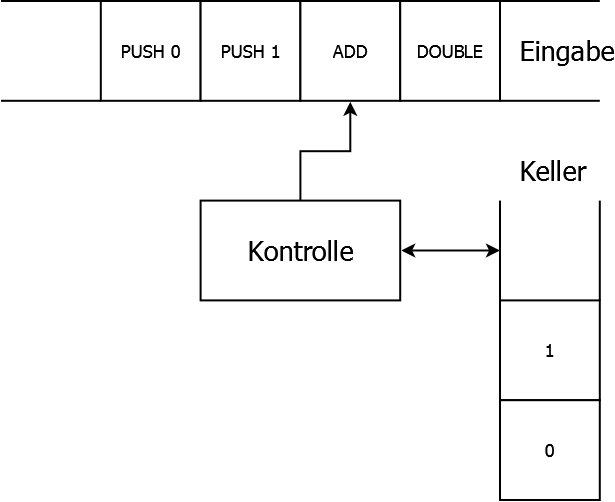
\includegraphics[width=240px]{../../gfx/einfacheKellermaschine.png}
	\caption{Einfacher Kellerautomat}\label{gfx:ekeller}
\end{figure}
%\textbf{Anmerk. v. Tobi:} \emph{Kontrolle in Abb. \ref{gfx:ekeller} ist eventuell ungünstig gewählt, bitte mal prüfen und ggf. mit DIA ändern.}\\
%Der Grundzustand $Z$ der Kellermaschine besteht also aus $<E_0|K_0>$. Für den Befehlssatz lassen sich folgende Zustandsveränderungsfunktion $\Delta$ definieren:
%\begin{align*}
%<\text{\lstinline!Push 0!}.\epsilon|\epsilon> &= <\epsilon|0.\epsilon>\\
%<\text{\lstinline!Push 1!}.\epsilon|\epsilon> &= <\epsilon|1.\epsilon>\\
%<\text{\lstinline!Read!}.\epsilon|x.\epsilon> &= <\epsilon|\epsilon>\\
%<\text{\lstinline!Add!}.\epsilon|y.x.\epsilon> &= <\epsilon|y+x.\epsilon>\\
%<\text{\lstinline!Sub!}.\epsilon|y.x.\epsilon> &= <\epsilon|y-x.\epsilon>\\
%<\text{\lstinline!Double!}.\epsilon|x.\epsilon> &= <\epsilon|x+x.\epsilon>\\
%\end{align*}

Grundzustand der in Abb. \ref{gfx:ekeller} dargestellten Kellermaschine ist $\langle K_0|S|E_0\rangle$\\
$\langle K_0|S|E_0\rangle\xrightarrow{Push\ 0} \langle 0.K|S|E_0\rangle$\\
$\langle K_0|S|E_0\rangle\xrightarrow{Push\ 1} \langle 1.K|S|E_0\rangle$\\
$\langle K_0|S|n.E_0\rangle\xrightarrow{Read} \langle n.K|S|E_0\rangle$, für alle $n\in N$\\
$\langle n_1.n_2.K_0|S|E_0\rangle\xrightarrow{Add} \langle n_1+n_2.K|S|E_0\rangle$, für alle $n_1,n_2\in N$\\
$\langle n_1.n_2.K_0|S|E_0\rangle\xrightarrow{Sub} \langle n_1-n_2.K|S|E_0\rangle$, für alle $n_1,n_2\in N$\\
$\langle n.K_0|S|E_0\rangle\xrightarrow{Double} \langle 2\cdot n.K|S|E_0\rangle$, für alle $n\in N$\\

Die Ergebnisse der Operationen (\lstinline!Add, Sub, Double!) liegen nach Ausführung des Befehls an erster Stelle auf dem Stack. Wenn eine Operation zwei Operanden verwendet wird das erste und das darunter liegende zweite Element verwendet.\\
\textbf{Anmerk. v. Tobi:} \emph{Das ist meine grobe Idee, da fehlt vermutlich noch ein Ausgabezustand in $<E_0|K_0>$, also eher etwas wie $<A_0|E_0|K_0>$.\\ ich sehe gerade das ich die Reihenfolge von Stack und Eingabe vertauscht habe, sollte aber kein großes Problem sein, bei mir steht einfach die Eingabe an erster Stelle.}\\
\section*{Aufgabe 3}
Formalisieren Sie Ihre Semantik aus Aufgabe 1 durch Angabe eines Interpreters bzgl. einer abstrakten Maschine mit dem Zustandsraum: $STACK \times KONTROLLE \times EINGABE$.\\

\begin{itemize}
	\item \textbf{Anfangszustand:}\\
		$Z_{T,S,E} = \langle\epsilon|S|T.\epsilon|E\rangle$\\
	\item \textbf{Zustandsüberführungsfunktion $\Delta$:}\\
		$\Delta$ induktiv über die Struktur der Kontrollkellerspitze:\\

		$\Delta (W|S|n.K|E) := \langle n.W|S¦K¦E\rangle$ für $n \in N$\\
		$\Delta (W|S|\underline{read}.K|n.E) := \langle n.W|S|K|E\rangle$ für $n \in N$\\
		$\Delta (W|S|T_1 \underline{OP} T_2.K|E) := \langle W|S|T_1.T_2.\underline{OP}.K|E\rangle$\\
		$\Delta (n_2.n_1.W|S|\underline{OP}.K|E) := \langle \underline{n_1\underline{OP}n_2}.W|S|K|E\rangle$ für $n_1,n_2 \in N$\\

		%TODO: prüfen ob evtl auch noch nötig ist:
		$\Delta (W|S|ND.K|E) := \langle W|S|N.N.+.D.+K|E\rangle$%(baut aus binären NDs die entsprechende Dezimalzahl)\\

\end{itemize}
\end{document}
